\documentclass[12pt]{article}
\usepackage[utf8]{inputenc}
\usepackage[portuguese]{babel}
\usepackage{graphicx}
\usepackage{booktabs}
\usepackage{array}
\usepackage{amsmath}
\usepackage{listings}
\usepackage{xcolor}
\usepackage{caption}
\usepackage{float}
\usepackage[top=2cm, bottom=2cm, left=2cm, right=2cm]{geometry}
\usepackage{titlesec}

\definecolor{codegreen}{rgb}{0,0.6,0}
\definecolor{codegray}{rgb}{0.5,0.5,0.5}
\definecolor{codepurple}{rgb}{0.58,0,0.82}
\definecolor{backcolour}{rgb}{0.95,0.95,0.92}

\lstdefinestyle{mystyle}{
	backgroundcolor=\color{backcolour},
	commentstyle=\color{codegreen},
	keywordstyle=\color{magenta},
	numberstyle=\tiny\color{codegray},
	stringstyle=\color{codepurple},
	basicstyle=\ttfamily\footnotesize,
	breakatwhitespace=false,
	breaklines=true,
	captionpos=b,
	keepspaces=true,
	numbers=left,
	numbersep=5pt,
	showspaces=false,
	showstringspaces=false,
	showtabs=false,
	tabsize=2,
	literate=%
	{á}{{\'a}}1 {é}{{\'e}}1 {í}{{\'i}}1 {ó}{{\'o}}1 {ú}{{\'u}}1
	{Á}{{\'A}}1 {É}{{\'E}}1 {Í}{{\'I}}1 {Ó}{{\'O}}1 {Ú}{{\'U}}1
	{à}{{\`a}}1 {è}{{\`e}}1 {ì}{{\`i}}1 {ò}{{\`o}}1 {ù}{{\`u}}1
	{À}{{\`A}}1 {È}{{\'E}}1 {Ì}{{\`I}}1 {Ò}{{\`O}}1 {Ù}{{\`U}}1
	{ä}{{\"a}}1 {ë}{{\"e}}1 {ï}{{\"i}}1 {ö}{{\"o}}1 {ü}{{\"u}}1
	{Ä}{{\"A}}1 {Ë}{{\"E}}1 {Ï}{{\"I}}1 {Ö}{{\"O}}1 {Ü}{{\"U}}1
	{â}{{\^a}}1 {ê}{{\^e}}1 {î}{{\^i}}1 {ô}{{\^o}}1 {û}{{\^u}}1
	{Â}{{\^A}}1 {Ê}{{\^E}}1 {Î}{{\^I}}1 {Ô}{{\^O}}1 {Û}{{\^U}}1
	{ã}{{\~a}}1 {ẽ}{{\~e}}1 {ĩ}{{\~i}}1 {õ}{{\~o}}1 {ũ}{{\~u}}1
	{Ã}{{\~A}}1 {Ẽ}{{\~E}}1 {Ĩ}{{\~I}}1 {Õ}{{\~O}}1 {Ũ}{{\~U}}1
	{ç}{{\c c}}1 {Ç}{{\c C}}1
}

\lstset{style=mystyle}

\titleformat{\section}{\normalfont\Large\bfseries}{\thesection}{1em}{}
\titleformat{\subsection}{\normalfont\large\bfseries}{\thesubsection}{1em}{}

\begin{document}

\thispagestyle{empty}

\begin{center}
	\begin{figure}[h]
		\centering
		
\includegraphics[width=0.35\textwidth]{images/logo_icmc.png}
	\end{figure}
	{\large\textbf{Universidade de São Paulo}}\\[1mm]
	{\large\textbf{Instituto de Ciências Matemáticas e de Computação}}\\[1mm]
	{\large\textbf{Departamento de Sistemas de Computação}}

	\vfill
	\large \textbf{SSC0902 - Organização e Arquitetura de Computadores}
	\vfill

	{\large Docente: Sarita Mazzini Bruschi}\\
	{\large Monitora: Catarina Moreira Lima}\\
	\vfill

	{\large\MakeUppercase{\textbf{Trabalho Prático 1: Calculadora Sequencial}}}
	\vfill
\end{center}

\begin{center}
	Gabriel Barbosa de Oliveira - gabriel\_barbosa@usp.br - 12543415 \\
	Laura Fernandes Camargos - laura.camargos@usp.br - 13692334 \\
	Sandy da Costa Dutra - sandycdutra@usp.br - 12544570 \\
	Nicholas Eiti Dan - nicholas.dan@usp.br - 14600749 \\
\end{center}

\begin{center}
	São Carlos, \today
\end{center}

\newpage

\pagestyle{plain}

\section{Objetivo}
O objetivo deste trabalho foi implementar uma calculadora sequencial
em Assembly RISC-V que realiza operações aritméticas básicas (adição,
subtração, multiplicação e divisão inteira) com funcionalidades
adicionais de desfazer operações (undo) e finalização do programa. O
projeto visou consolidar os conhecimentos sobre programação em
Assembly, manipulação de registradores, controle de fluxo e
estruturas de dados, especialmente listas encadeadas.

\section{Descrição Geral do Programa}
A calculadora desenvolvida opera em um loop contínuo, solicitando
inicialmente um número e, em seguida, uma operação. As operações suportadas são:
\begin{itemize}
	\item \textbf{+}: Adição
	\item \textbf{-}: Subtração
	\item \textbf{*}: Multiplicação
	\item \textbf{/}: Divisão inteira (com tratamento de divisão por zero)
	\item \textbf{u}: Desfaz a última operação (undo)
	\item \textbf{f}: Finaliza o programa
\end{itemize}

Cada resultado é armazenado em uma lista encadeada, permitindo que a
operação \textbf{u} (undo) restaure o estado anterior da calculadora.
O programa também inclui tratamento de erros para operações
inválidas, números malformados e divisões por zero.

\section{Estratégia Adotada}
\subsection{Registradores}
Os registradores foram utilizados conforme a convenção do RISC-V:
\begin{itemize}
	\item \textbf{s0}: Armazena o resultado atual das operações.
	\item \textbf{a0, a1}: Usados para passagem de parâmetros e retorno de valores.
	\item \textbf{t0-t6}: Registradores temporários para cálculos intermediários.
	\item \textbf{ra}: Armazena o endereço de retorno para chamadas de função.
\end{itemize}

\subsection{Lista Encadeada}
A lista encadeada armazena os resultados das operações.\\
Cada nó da lista contém:
\begin{itemize}
	\item \textbf{4 bytes}: Valor do resultado.
	\item \textbf{4 bytes}: Ponteiro para o próximo nó (ou -1 para NULL).
\end{itemize}

A label \textbf{store\_result} aloca dinamicamente um novo nó e o
adiciona no início da lista. A label \textbf{undo} remove o nó
mais recente e restaura o valor anterior.

\subsection{Tratamento de Erros}
Foram implementadas mensagens de erro específicas para:
\begin{itemize}
	\item Divisão por zero.
	\item Operação inválida.
	\item Número inválido.
	\item Tentativa de desfazer operação quando não há operações anteriores.
\end{itemize}

\section{Principais trechos de código}
\subsection{Leitura e validação dos números inteiros}
\begin{lstlisting}[language={[x86masm]Assembler}, caption=Leitura e validação de números completos]
read_valid_integer:
    addi sp, sp, -16             # Reserva espaço na pilha
    sw ra, 0(sp)                 # Salva endereço de retorno
    sw s0, 4(sp)                 # Salva registradores salvos
    sw s1, 8(sp)
    sw s2, 12(sp)

read_integer_again:
    li a7, 4
    la a0, number_prompt
    ecall

    # Lê string do usuário
    li a7, 8
    la a0, input_buffer
    li a1, 16                    # Tamanho máximo da entrada
    ecall

    la s0, input_buffer          # s0 = ponteiro para a string
    li s1, 0                     # s1 = sinal (0=+, 1=-)
    li s2, 0                     # s2 = contador de dígitos
    li t2, 0                     # t2 = valor acumulado
    li t3, 10                    # t3 = base decimal (10)

    # Verifica sinal negativo
    lb t0, 0(s0)                 # Carrega primeiro caractere
    li t1, '-'
    bne t0, t1, check_first_digit
    li s1, 1                     # Marca como negativo
    addi s0, s0, 1               # Avança para próximo caractere

check_first_digit:
    lb t0, 0(s0)                 # Primeiro caractere após sinal
    li t1, 10                    # ASCII para newline
    beq t0, t1, invalid_input    # String vazia
    li t1, '0'
    blt t0, t1, invalid_input    # Caractere menor que '0'
    li t1, '9'
    bgt t0, t1, invalid_input    # Caractere maior que '9'

process_digits:
    lb t0, 0(s0)                 # Carrega próximo caractere
    li t1, 10                    # ASCII para newline
    beq t0, t1, validation_done  # Fim da string

    # Verifica se é dígito (0-9)
    li t1, '0'
    blt t0, t1, invalid_input
    li t1, '9'
    bgt t0, t1, invalid_input

    # Converte ASCII para valor numérico
    addi t0, t0, -48             # Converte '0'-'9' para 0-9

    # Multiplica acumulador por 10 e adiciona novo dígito
    mul t2, t2, t3               # t2 = t2 * 10
    add t2, t2, t0               # t2 = t2 + dígito_atual

    addi s0, s0, 1               # Próximo caractere
    addi s2, s2, 1               # Incrementa contador
    li t4, 11                    # Máximo de dígitos
    bge s2, t4, invalid_input    # Número muito grande
    j process_digits

validation_done:
    # Verifica se teve pelo menos 1 dígito
    beqz s2, invalid_input

    # Aplica sinal negativo se necessário
    beqz s1, positive_number
    neg t2, t2

positive_number:
    mv a0, t2                    # Retorna valor convertido
    lw ra, 0(sp)                 # Restaura registradores
    lw s0, 4(sp)
    lw s1, 8(sp)
    lw s2, 12(sp)
    addi sp, sp, 16
    jr ra

invalid_input:
    li a7, 4                     # Mostra mensagem de erro
    la a0, invalid_number_error
    ecall

    j read_integer_again         # Volta a pedir o número
\end{lstlisting}

\textbf{Explicação detalhada}:
\begin{enumerate}
	\item \textbf{Estrutura}:
		\begin{itemize}
			\item A função começa salvando registradores importantes na pilha
			\item Exibe um prompt solicitando a entrada do usuário
		\end{itemize}

	\item \textbf{Processamento}:
		\begin{itemize}
			\item Lê a string de entrada do usuário para um buffer
			\item Verifica se o primeiro caractere é '-' para números negativos
			\item Percorre cada caractere validando se é um dígito (0-9)
		\end{itemize}

	\item \textbf{Conversão}:
		\begin{itemize}
			\item Converte cada caractere ASCII para seu valor numérico
			\item Constrói o número final multiplicando por 10 e somando cada novo dígito
			\item Limita a 10 dígitos para evitar overflow
		\end{itemize}

	\item \textbf{Tratamento de erros}:
		\begin{itemize}
			\item Rejeita entradas vazias
			\item Rejeita caracteres não numéricos
			\item Rejeita números muito longos
			\item Mostra mensagem de erro específica e repete a solicitação
		\end{itemize}

	\item \textbf{Finalização}:
		\begin{itemize}
			\item Aplica o sinal negativo se necessário
			\item Retorna o valor convertido em a0
			\item Restaura todos os registradores antes de retornar
		\end{itemize}
\end{enumerate}

\textbf{Características da implementação}:

\begin{itemize}
	\item Aceita números positivos e negativos
	\item Verifica cada dígito individualmente
	\item Limita o tamanho máximo do número
	\item Fornece feedback claro em caso de erro
	\item Mantém a consistência mesmo com entradas inválidas
\end{itemize}

\begin{figure}[H]
	\centering
	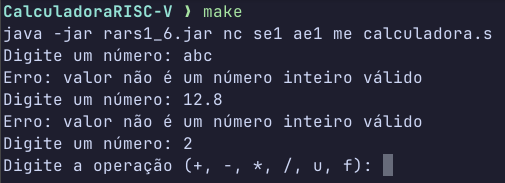
\includegraphics[width=0.6\textwidth]{images/input_validation.png}
	\caption{Exemplo de validação de entrada}
\end{figure}

\subsection{Lista Encadeada}

\begin{lstlisting}[language={[x86masm]Assembler}, caption=Armazenamento de resultados]
store_result:
    mv t0, a0           # Salva o valor a ser armazenado

    # Aloca memória para novo nó
    li a0, 8            # Tamanho do nó (8 bytes)
    li a7, 9            # Código de syscall para alocação
    ecall

    # Configura novo nó
    sw t0, 0(a0)        # Armazena o resultado
    lw t1, list_head    # Pega endereço atual da cabeça
    sw t1, 4(a0)        # Armazena como próximo nó

    # Atualiza cabeça da lista
    la t2, list_head
    sw a0, 0(t2)        # Novo nó é agora a cabeça
    jr ra
\end{lstlisting}

\textbf{Explicação}: Implementação da lista encadeada que armazena os
resultados das operações para permitir o undo. Cada nó contém o valor
e um ponteiro para o próximo nó.

\subsection{Operação Undo}

\begin{lstlisting}[language={[x86masm]Assembler}, caption=Implementação do undo]
undo_operation:
    la t0, list_head
    lw t1, 0(t0)        # Pega cabeça atual
    beq t1, s11, undo_error_case

    lw t2, 4(t1)        # Pega próximo nó
    beq t2, s11, undo_last_operation

    sw t2, 0(t0)
    lw s0, 0(t2)        # Restaura resultado anterior
    jr ra
\end{lstlisting}

\textbf{Explicação}: A função remove o nó mais recente da lista e
restaura o valor anterior, tratando casos especiais quando não há
operações para desfazer.

\begin{figure}[H]
	\centering
	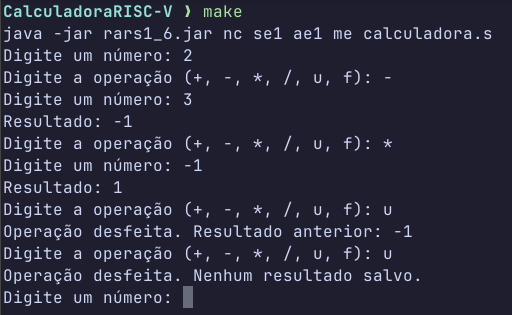
\includegraphics[width=0.6\textwidth]{images/undo_operation.png}
	\caption{Exemplo da operação undo em execução}
\end{figure}

\section{Exemplos de Execução}

\subsection{Operações Básicas}

\begin{figure}[H]
	\centering
	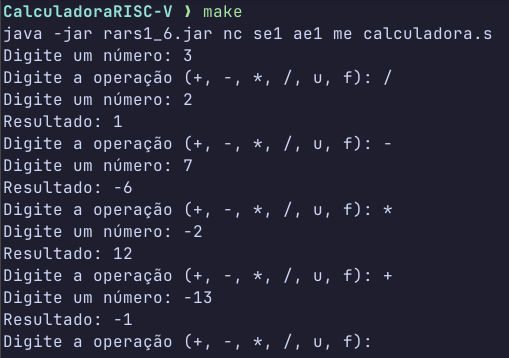
\includegraphics[width=0.6\textwidth]{images/basic_operations.png}
	\caption{Execução de operações aritméticas básicas}
\end{figure}

\subsection{Tratamento de Erros}

\begin{figure}[H]
	\centering
	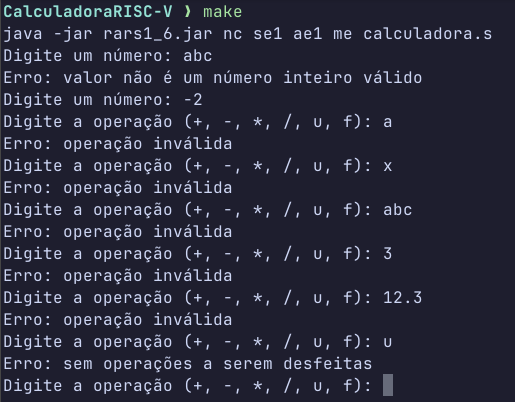
\includegraphics[width=0.6\textwidth]{images/error_handling.png}
	\caption{Exemplos de tratamento de erros}
\end{figure}

\section{Dificuldades Encontradas}
\begin{itemize}
	\item \textbf{Manipulação de Strings}: A leitura e validação de
		números como strings demandou atenção especial para tratar
		caracteres inválidos e sinais negativos.
	\item \textbf{Gerenciamento de Memória}: A implementação da lista
		encadeada exigiu cuidado com a alocação de nós para
		evitar acessos indevidos e erros.
	\item \textbf{Tratamento de Erros}: O tratamento de input
		inadequado do usuário foi um desafio e adicionou complexidade
		extra ao código.
	\item \textbf{Liberação da Memória não usada}: Não é o caso com
        o simulador, mas em uma aplicação real, a memória alocaad na
        heap precisaria ser liberada quando o nó não fosse
        mais utilizado.
\end{itemize}

\section{Conclusão}
O projeto foi concluído com sucesso, atendendo a todos os requisitos
especificados. A calculadora demonstra eficiência na execução das
operações básicas e na manipulação da lista encadeada para a
funcionalidade de undo. As dificuldades encontradas foram superadas
e a robustez do programa foi confirmada nos testes.

\end{document}
